% 
% Template file for software architecture design description in the 
% DIKU course Software Architecture and Software Design. Please do
% not distribute outside the course
% 
% Based on a template (c) by Woods and Rozanski (2011) available at
% 
%    http://www.viewpoints-and-perspectives.info
% 
% Instructions:
%
% 1) change the metadata commands below (\groupname) etc. to fit your
%     project
% 2) uncomment the overwriting of the \instructions command to remove 
%     instructions
% 3) write your architectural description...
%
% Contact: klausmh@diku.dk
% 
\documentclass[a4paper,11pt]{report}
\usepackage{natbib}
\usepackage[pdftex]{graphicx}
\usepackage{color}
\usepackage[table]{xcolor}
\usepackage{hyperref}
\usepackage{lastpage} 
\usepackage{rotating}
\usepackage{longtable}

% Meta-data for report
\newcommand{\systemname}{Siberian Trucking System}
\newcommand{\groupname}{Lima}
\newcommand{\contactdetails}{athas@sigkill.dk, shantanubala@gmail.com, jesper\_tved@hotmail.com}

% Typesetting of instructions for using the template,
% remove by renewing command 
\newcommand{\instructions}[1]{
  \noindent\colorbox{lightgray}{%
    \parbox{\linewidth}{%
      #1
    }%
  }%
 \vspace{0.1cm}
}
% \renewcommand{\instructions}[1]{} % Uncomment to remove instructions

% We use the below command for figure captions since
% the figure environment does not play nicely with 
% \colorbox. The "real" way to create figures is like this:
%   \begin{figure}[ht!]
%     \centering
%     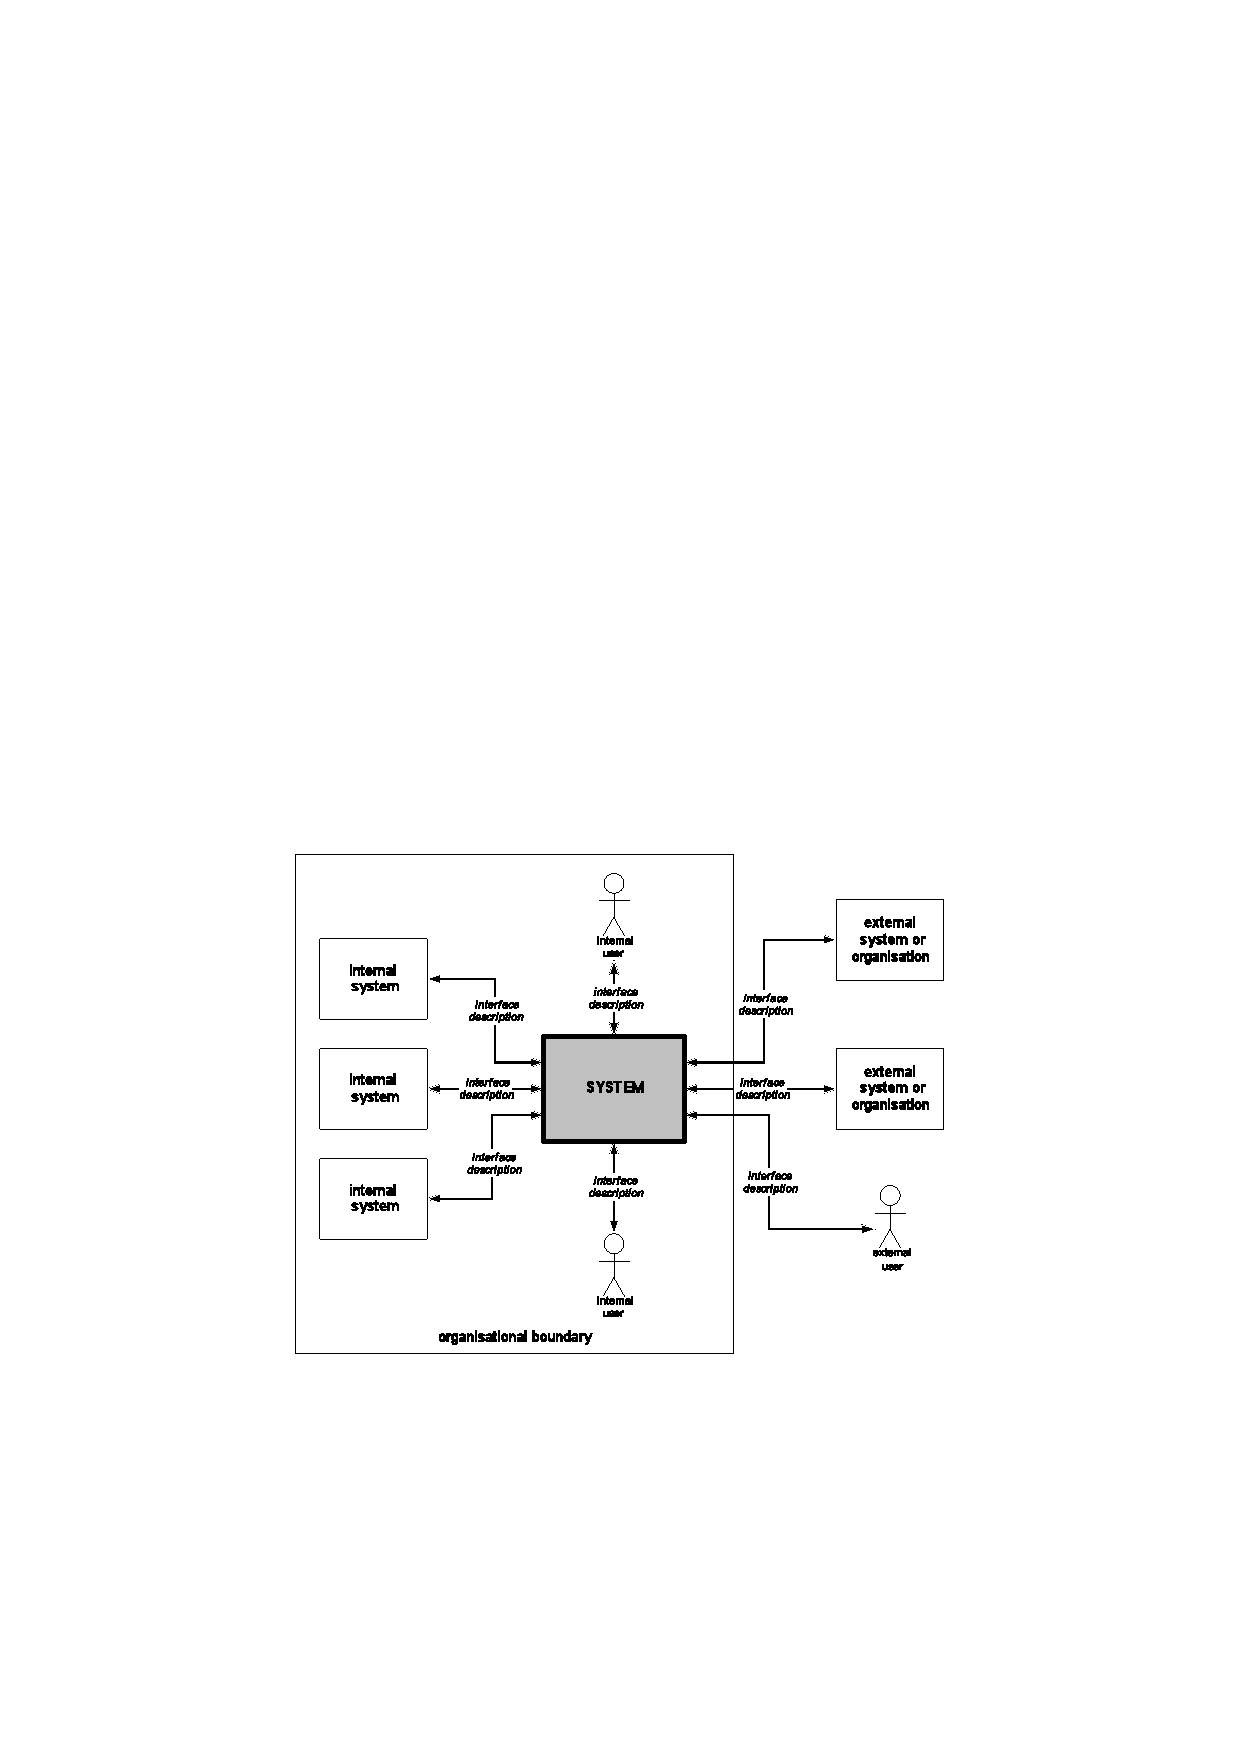
\includegraphics[width=0.8\textwidth]{figures/systemcontext}
%    \caption{System context}
%     \label{fig:systemcontext}
%   \end{figure}
\newcommand{\mycaption}[1]{
  \addtocounter{figures}{1}
  Figure \arabic{figures}. #1
}

% Change font family to Helvetica
\renewcommand{\rmdefault}{phv}
\renewcommand{\sfdefault}{phv}

% Set headers and footers
\usepackage{fancyhdr}
\pagestyle{fancy}
\fancyhf{}
\fancyhead[C]{Software Architecture of \systemname\ }
\fancyfoot[C]{\footnotesize Page \thepage\ of \pageref{LastPage}}


\begin{document}
% 
% Title page
% 
\newcommand{\HRule}{\rule{\linewidth}{0.5mm}}
\begin{titlepage}

  \begin{center}

    % Title
    \vspace*{4cm}
    \HRule \\[0.4cm]
    { \huge \bfseries \systemname}\\[0.4cm]
    \HRule \\[1.5cm]

    {\Large Software Architecture Description}

    \vfill
  \end{center}

  % Author, version, date
  \begin{flushleft}
    {\large \groupname}\\[0.2cm]
    {\large \contactdetails}\\[0.2cm]
   {\large \today}
  \end{flushleft}
\end{titlepage}

% 
% Version table
% 
\newpage
\chapter*{Version history}

\begin{center}
  \begin{tabular}[h!]{| l | l | l | p{8 cm} |}
    \hline
    \rowcolor{gray}
    Version & Date & Author & Comments \\
    \hline
    \hline
    1 & 2012-08-17 & KMH & Initial template based on
    \citep{rozanski2011software} \\
    \hline
    3 & 2012-09-17 & SHB and JTM & added chapter 3\\
    \hline
    4 & 2012-09-19 & TRH, SHB and JTK & Revised 3.1, clarified truck transmitter concept \\
    \hline
    5 & 2012-09-24 & TRH, SHB and JTM & added chapter 4 and 5.2\\
    \hline
    6 & 2012-10-08 & TRH, SHB and JTM & added chapter 5 \\
    \hline
    7 & 2012-10-10 & TRH, SHB and JTM & Added sections 6 and 6.1\\
   \hline
  \end{tabular}
\end{center}

% 
% Table of contents
% 
\setcounter{tocdepth}{1}
\tableofcontents

% 
% Main text
% 
\chapter{Introduction}
\label{cha:introduction}
\thispagestyle{fancy}

\section{Purpose and scope}
\label{sec:purpose-scope}

Russia, as the worlds largest country by land area, has an extensive
raw materials industry.  Since the fall of the Soviet Union, the
Russian trucking industry has undergone a dramatic growth, and
government initiatives aim to maintain this growth into the future.
Since many of the industrial installations are located in remote
areas, logistics companies face great difficulties in managing their
truck fleets, particularly as transportation times are often
unpredictable due to weather, accidents and the generally poor
condition of the Russian road network.  As an additional complication,
the distant locations and low population densities prevents the use of
many common communication technologies (eg. no cell phone network).

We propose the creation of a system, the Siberian Tracking System
(STS), for tracking a large fleet of trucks operating in far-flung
regions of Russia, owned by the (fictive) Siberian Trucking Company
(STC).  A central server installation will be informed of the location
and state of every truck in the fleet, permitting decision making
systems to have complete knowledge of the state of the company assets.
Each truck is responsible for tracking its own progress, then
periodically relaying it back to the main servers.  The project does
not involve creation of any new ground stations; trucks will use
standard wireless communication methods whenever in range of
appropriate networks. The transmitters on the trucks will only use one way communication to the server, with data of the trucks current position and the speed of the truck. The transmitters are supposed to be low-cost hardware, so communication from the server to the trucks and additional measuring equipment, for instance of oil and gasoline levels have been deselected. 

The STS is solely concerned with the state of the trucking fleet, and
does not do freight tracking or make any kind of business logic
decisions on its own.  While it provides information allowing such
decisions to be made, it is purely a data collection and dissemination
infrastructure.  In particular, it is a one-way communication system.
Other means must be employed to contact the trucks on the road.  Also,
STS is by itself not concerned with doing data mining or presenting a
sophisticated user interface to its data.  Instead, a data interchange
mechanism will be defined that allows other systems to receive
information from STS.

\section{Audience}
\label{sec:audience}

The intended audience of this document, and the reason for their
inclusion, are as follows.

\begin{itemize}
  \item Business logic decision makers of STC, who must determine
    whether the information provided by STS is sufficient.
  \item Truck maintenance department representatives, to determine
    whether the additional equipment needed on trucks is realistic.
  \item The developers who have to implement the suggested architecture and design.
  \item Finally, whoever approves the financing of the project.
\end{itemize}

\section{Status}
\label{sec:status}

The basic requirements and design of STS has been determined, but the
actual implementation has not yet begun.

\section{Architectural design approach}
\label{sec:arch-design-appr}

\chapter{Glossary}
\label{cha:glossary}
\thispagestyle{fancy}

\begin{center}
  \begin{tabular}[h!]{| p{0.2\textwidth} | p{0.7\textwidth} |}
    \hline
    \rowcolor{gray}
    Term & Definition \\
    \hline
    \hline
    Canonical truck position & An externally registered position of a specific truck at a specific time.  Used to check consistency with measured positions. \\\hline
    Mesh network & An ad-hoc (usually short-range) network formed by autonomous units within range of each other \\\hline
    STS & Siberian Tracking System.  Refers both to the project as a whole, and to the software running on stationary servers (ie. excluding the software on truck transmitters). \\\hline
    STC & Siberian Tracking Company \\\hline
    Truck transmitter & The hardware unit on a truck.  Consists of a GPS receiver and an antenna for communications. \\\hline
    AWS & Amazon Web Services - the cloud computing platform chosen for the STS. \\\hline
  \end{tabular}
\end{center}

\chapter{System stakeholders and requirements}
\label{cha:syst-stak-requ}
\thispagestyle{fancy}

\section{Stakeholders}
\label{sec:stakeholders}

\begin{itemize}
  \item Acquirers: the Siberian Trucking Company (STC) will be paying for the
    development of the system to aid in business logic. The users of the system
    will be members of the STC's business administration.
  \item Communicators: the technical writers who will create documentation regarding the
    operation of the system, while the business administration of the STC will
    be responsible for the training of the end users of the system.
  \item Developers: the STC has contracted a group from the University of
    Copenhagen to develop the system.
  \item Maintainers: the STC has a team of developers responsible for
    maintaining and evolving the STS system after it is completed.
  \item Production Engineers: the STS system will be deployed onto the Amazon
    EC2 platform, outsourcing the deployment environment to Amazon's
    engineering staff.
  \item Suppliers: servers will be provided by Amazon's EC2 platform, while the
    GPS units are assumed to already be installed on the STC's trucks.
  \item Support Staff: it is assumed that the STC has the appropriate IT staff
    for helping the end users of the STS in accomplishing their appropriate
    business administration tasks.
  \item System Administrators: Amazon provides the appropriate hardware
    administration while the STC has a team of developers responsible for
    updating and maintaining the software environment of the EC2 instances.
  \item Testers: The STC has a team of developers responsible for testing and
    ensuring the STS works effectively.
  \item Users: members of the STC's business administration team who will use
    and analyze data provided by the STS to make informed business decisions.
\end{itemize}

\section{Overview of requirements}
\label{sec:overv-requ}

\begin{center}
  \begin{tabular}[h!]{| p{0.2\textwidth} | p{0.7\textwidth} |}
    \hline
    \rowcolor{gray}
    Reference & Requirement description \\
    \hline
    \hline
    R1 & The system must provide business administrators with a detailed
    history of the location of every truck in the STC fleet. \\
    \hline
    R2 & The system must be able to receive and store 1,000 GPS datapoints per
    second. \\
    \hline
    R3 & The server interface for storing the trucks' location data must have
    an availability of at least 99 percent uptime. \\
    \hline
    R4 & The tracking units present on each of the trucks must have a fallback
    when data cannot be sent in real-time due to bad network coverage. \\
    \hline
    R5 & The server interface must be capable of receiving an individual data
    point (the truck's location) or a series of data points (the truck's
    location history over a period of time). \\
    \hline
  \end{tabular}
\end{center}

\section{System scenarios}
\label{sec:system-scenarios}

\subsection{Functional scenarios}
\label{sec:functional-scenarios}

\begin{center}
  \begin{tabular}[h!]{| >{\columncolor{gray}}p{0.28\textwidth} | p{0.65\textwidth} |}
    \hline
    Scenario reference & FS1. \\
    \hline
    Overview & How truck information is sent to the server \\
    \hline
    System state & The truck is fitted with a truck transmitter and is currently driving\\
    \hline
    System environment & The system is operating normally\\
    \hline
    External stimulus & The truck transmitter has a position that should be sent to the server\\
    \hline
    Required system response & If the truck is in range of a network, the position is sent to the server and a confirmation is received. If the truck is out of range, the position is stored in the truck transmitter and will be sent when the truck is in range of a network again \\
    \hline
  \end{tabular}
\end{center}

\begin{center}
  \begin{tabular}[h!]{| >{\columncolor{gray}}p{0.28\textwidth} | p{0.65\textwidth} |}
    \hline
    Scenario reference & FS2. \\
    \hline
    Overview & How truck positions are queried by a user \\
    \hline
    System state & Positions from many different trucks have been sent to the server with timestamps\\
    \hline
    System environment & The system is operating normally\\
    \hline
    External stimulus & The user queries a specific truck, trucks within an area, and trucks that have not yet reached their deignated targets on time\\
    \hline
    Required system response & The system shows the requested data as a list in the users GUI \\
    \hline
  \end{tabular}
\end{center}

\begin{center}
  \begin{tabular}[h!]{| >{\columncolor{gray}}p{0.28\textwidth} | p{0.65\textwidth} |}
    \hline
    Scenario reference & FS3. \\
    \hline
    Overview & New trucks are imported to the system \\
    \hline
    System state & New trucks are listed in the truck registry and a transmitter have been fitted into the new truck\\
    \hline
    System environment & STS, the truck transmitter and the truck registry is operating normally\\
    \hline
    External stimulus & An employee from the support staff have registered the truckID with the trucks transmitterID \\
    \hline
    Required system response & STS can now be queried for the new trucks ID \\
    \hline
  \end{tabular}
\end{center}

\begin{center}
  \begin{tabular}[h!]{| >{\columncolor{gray}}p{0.28\textwidth} | p{0.65\textwidth} |}
    \hline
    Scenario reference & FS4. \\
    \hline
    Overview & How transmittion network are chosen \\
    \hline
    System state & The truck is fitted with a truck transmitter and is currently driving\\
    \hline
    System environment & The truck transmitter and the truck registry is operating normally, the truck is driving in an area without any connection\\
    \hline
    External stimulus & The truck transmitter has a new position that should be sent to the server \\
    \hline
    Required system response & The truck transmitter first tries to send via GSM mobile network, after this the long range mesh-network is tried. If neither of these worked, the position is stored to be sent at a later point. \\
    \hline
  \end{tabular}
\end{center}

\subsection{System quality scenarios}
\label{sec:syst-qual-scen}

\begin{center}
  \begin{tabular}[h!]{| >{\columncolor{gray}}p{0.28\textwidth} | p{0.65\textwidth} |}
    \hline
    Scenario reference & QS1. \\
    \hline
    Overview & If the number of trucks in the fleet increases, or if the business
    administrators need to collect data at a greater interval, the capabilities
    of the system ought to be appropriately scalable.\\
    \hline
    System environment & This process will be handled
    by Amazon's Elastic Load Balancing service in conjunction with Amazon EC2.\\
    \hline
    Environment changes & For example, if 10 small EC2
    instances can receive and process 1,000 data points per second, the system will
    allocate the equivalent of 50 small EC2 instances to process an increased
    workload of 5,000 data points per second.\\
    \hline
    Required system behavior & When a tracking device in
    a truck sends data to the STS server, the data will be placed in a queue.
    Based on the size of the queue, an appropriate number of EC2 instances will
    be started or shut down to process the queue.\\
    \hline
  \end{tabular}
\end{center}

\begin{center}
  \begin{tabular}[h!]{| >{\columncolor{gray}}p{0.28\textwidth} | p{0.65\textwidth} |}
    \hline
    Scenario reference & QS2. \\
    \hline
    Overview & If the cellular network is not available, the transmitter on the
    truck will fall back to using a long-distance mesh network established
    between the trucks. \\
    \hline
    System environment & This process will be handled
    by the transmitters that are installed on every truck in the STC fleet.\\
    \hline
    Environment changes & For example, if a truck leaves cell network range, it
    will attempt to connect to a nearby truck, which will also be connected to
    other trucks. As long as a single truck in the mesh has cell coverage, all
    of the trucks will be able to transmit their data.\\
    \hline
    Required system behavior & The trucks' transmitters will have a queue for
    sending data to the STS server, and will process this queue using the
    fastest available connection.\\
    \hline
  \end{tabular}
\end{center}

\begin{center}
  \begin{tabular}[h!]{| >{\columncolor{gray}}p{0.28\textwidth} | p{0.65\textwidth} |}
    \hline
    Scenario reference & QS3. \\
    \hline
    Overview & If part of the Amazon EC2 cluster fails, the error must not propagate to the entire system.\\
    \hline
    System environment & This robustness must be built into the software running on the EC2 cluster.  Additionally, the truck transmitters must still be able to transmit data. \\
    \hline
    Environment changes & If a node in the cluster loses contact with another node, it must ensure that the overall system still has redundant data, such that further node failures can be handled.  The trucks must be able to connect to another node if the usual recipient for their data fails to respond.  If the system is sufficiently heavily damaged that data integrity is lost, it must still be possible for trucks to transmit data, but any queries in the data should have their result marked as incomplete.  \\
    \hline
    Required system behavior & Heavy data redundancy must be built into the system.  Whenever a truck reports back, it may also receive an updated list of communication endpoints. \\
    \hline
  \end{tabular}
\end{center}

\begin{center}
  \begin{tabular}[h!]{| >{\columncolor{gray}}p{0.28\textwidth} | p{0.65\textwidth} |}
    \hline
    Scenario reference & QS4. \\
    \hline
    Overview & If the transmitter on a truck fails, this failure must be noticed and rectified. \\
    \hline
    System environment & The system must have logic to detect when a truck ``should'' have transmitted information, but has not.  We assume that the fabrication and installation of new transmitters is done externally of our system. \\
    \hline
    Environment changes & If a truck fails to report back, the maintenance department must be notified that a truck has a faulty transmitter, and that it must be replaced. \\
    \hline
    Required system behavior & We receive information from the truck register whenever the truck reaches some central locations (the \textit{canonical truck position}).  If the truck itself does not send the same information, its transmitter will be assumed defective, and called in for repair.  As long as every truck is guaranteed to eventually stop at such a destination, any failure will eventually be discovered. \\
    \hline
  \end{tabular}
\end{center}

\chapter{Architectural forces}
\label{cha:architectural-forces}
\thispagestyle{fancy}

\section{Goals}
\label{sec:goals}

\begin{description}
\item[Business driver:] Trucking in Russia is mostly done using old and inefficient
  trucks with bad road conditions.  It is not feasible to replace the
  vehicles or the road system, so in order to remain competetive, the
  STC must optimise its logistics intead.
\item[Project goal:] The STC wishes to optimise its logistics by
  keeping a detailed log of truck movement.  By analysing the
  information the log, more efficient transportation routes may be
  designed.
\item[Project goal:] In order to minimise truck idle time, the STC
  desires real-time information on truck locations, such that
  availability for further use can be easily predicted.
\end{description}

\section{Constraints}
\label{sec:constraints}

\begin{itemize}
\item The company has very little in-house IT capacity, and does not
  wish to expand it much.  In particular, it does not want to maintain
  its own servers.
\item Since the servers must consequently be outsourced, the STS has
  to run in a generic, non-customised environment (such as a standard
  Linux server).
\item The truck transmitters are very restricted, embedded hardware,
  that cannot run large and complicated software.
\item Trucking in Russia is at an unusually high risk of hijacking.
  In order to not leak information about the locations of trucks, all
  communications has to be protected from eavesdropping, and all
  queries in the database must be authorised.
\item As another safety-related concern, it must not be possible for a
  third party to falsify truck information.
\end{itemize}

\section{Architectural principles}
\label{sec:arch-princ}

\begin{center}
  \begin{tabular}[h!]{| >{\columncolor{gray}}p{0.28\textwidth} | p{0.65\textwidth} |}
    \hline
    Principle reference & P1. \\
    \hline
    Principle statement & Redundancy of components \\
    \hline
    Rationale & The STS will be of critical importance in making real-time business decisions, so it is important that it is always available. \\
    \hline
    Implications & \begin{itemize}
      \item System distributed across multiple nodes (for example, using multiple different Amazon EC2 instances across multiple availability zones).
      \item Comprehensive error handling in all levels of the system.
      \item Load balancing to handle node failures.
      \item Redundancy at the data level, for example through replication.
      \end{itemize}
        \\
    \hline
  \end{tabular}
\end{center}
\begin{center}
  \begin{tabular}[h!]{| >{\columncolor{gray}}p{0.28\textwidth} | p{0.65\textwidth} |}
    \hline
    Principle reference & P2. \\
    \hline
    Principle statement & Use of open source components \\
    \hline
    Rationale & Open source components will be used where available, in order to reduce development effort and cost. \\
    \hline
    Implications & \begin{itemize}
      \item Able to modify external components, if necessary.
      \end{itemize}
        \\
    \hline
  \end{tabular}
\end{center}
\begin{center}
\begin{tabular}[h!]{| >{\columncolor{gray}}p{0.28\textwidth} | p{0.65\textwidth} |}
    \hline
    Principle reference & P3. \\
    \hline
    Principle statement & Encryption of communications \\
    \hline
    Rationale & To prevent outsiders from gaining knowledge about truck locations, all communications across external networks must be encrypted \\
    \hline
    Implications & \begin{itemize}
      \item An encryption scheme must be decided upon.
      \item We don't have to worry about security of the link layers.
      \end{itemize}
        \\
    \hline
  \end{tabular}
\end{center}
\begin{center}
\begin{tabular}[h!]{| >{\columncolor{gray}}p{0.28\textwidth} | p{0.65\textwidth} |}
    \hline
    Principle reference & P4. \\
    \hline
    Principle statement & Cryptographic signing of truck communications \\
    \hline
    Rationale & To prevent third parties from impersonating truck transmitters, all communications from trucks must be signed using assymetric cryptography. \\
    \hline
    Implications & \begin{itemize}
    \item The cryptographic keys must be managed.
    \item If a key is leaked, there must be a procedure for changing them.
    \end{itemize}
        \\
    \hline
  \end{tabular}
\end{center}
\begin{center}
\begin{tabular}[h!]{| >{\columncolor{gray}}p{0.28\textwidth} | p{0.65\textwidth} |}
    \hline
    Principle reference & P5. \\
    \hline
    Principle statement & The information retrieval API is REST-oriented \\
    \hline
    Rationale & REST APIs are easy to interface with existing HTTP protocol stacks. \\
    \hline
    Implications & \begin{itemize}
    \item We need visible HTTP servers.
    \item A protocol for how to represent the data in textual form
      must be decided.
    \end{itemize}
        \\
    \hline
  \end{tabular}
\end{center}

\begin{center}
\begin{tabular}[h!]{| >{\columncolor{gray}}p{0.28\textwidth} | p{0.65\textwidth} |}
  \hline
  Principle reference & P6. \\
  \hline
  Principle statement & Mesh networking by trucks \\
  \hline
  Rationale & In order to extend range beyond cell phone networks, short-range mesh networks between truck transmitters is used to indirectly transmit to STS. \\
  \hline
  Implications & \begin{itemize}
  \item A truck can relay information about any number of other trucks.
  \item Every piece of truck communication must be identified by the
    original sender, not the truck that managed to contact the STS.
    \end{itemize}
        \\
    \hline
  \end{tabular}

\end{center}

\chapter{Architectural views}
\label{cha:architectural-views}
\thispagestyle{fancy}

\section{Context view}
\label{sec:context-view}

\newcounter{figures}

\begin{center}
  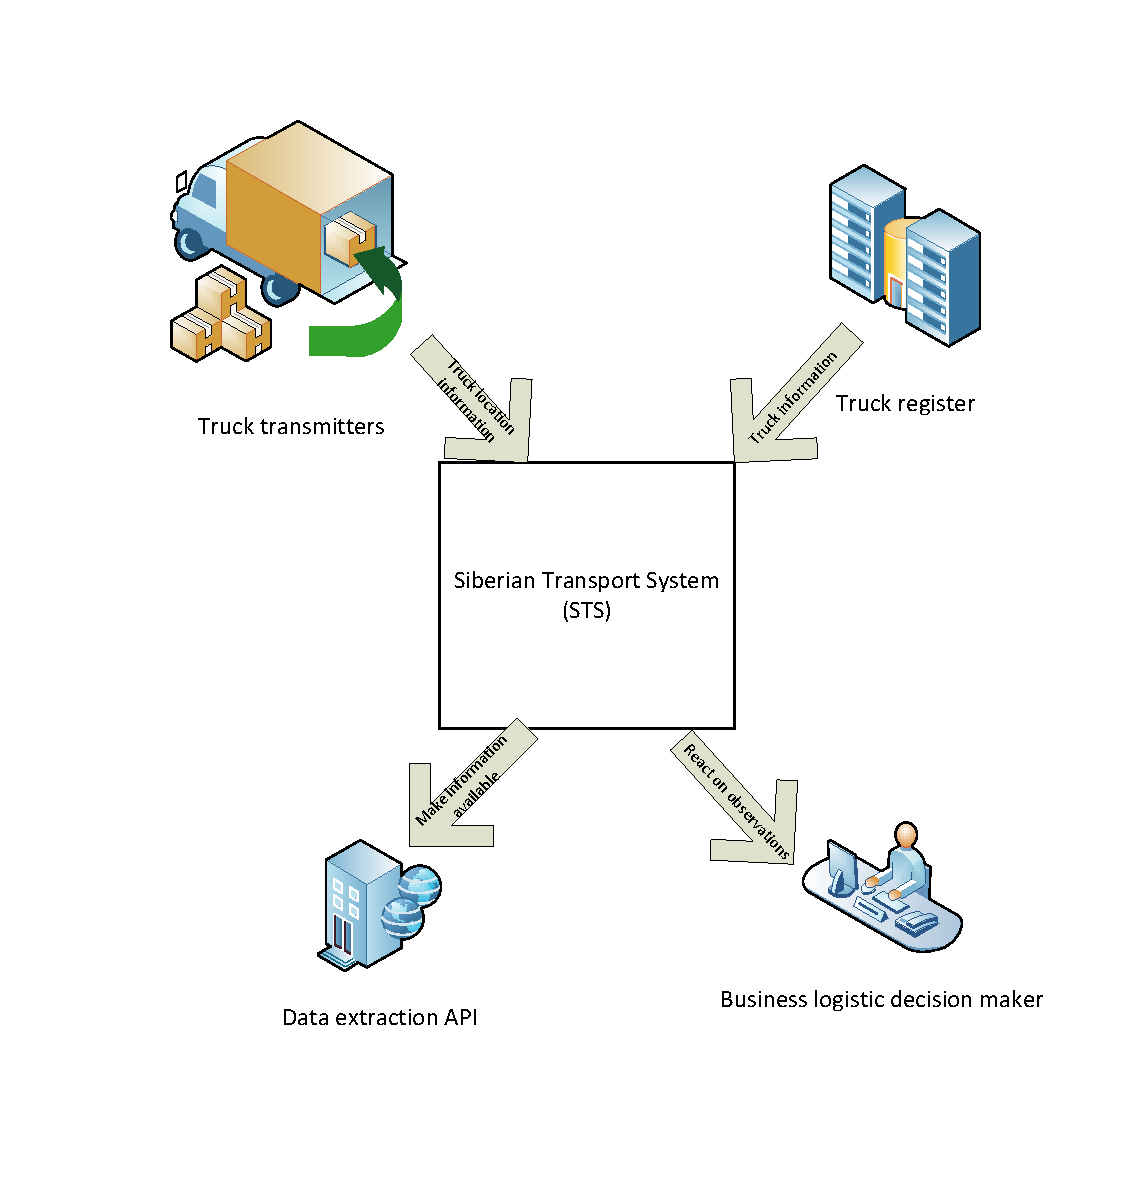
\includegraphics[width=\textwidth]{figures/sts_context_view}\\
\end{center}
  \mycaption{Context diagram of the Siberian Transport System (STS) }

\subsection{Context diagram}
\label{sec:context-diagram}

\begin{center}
  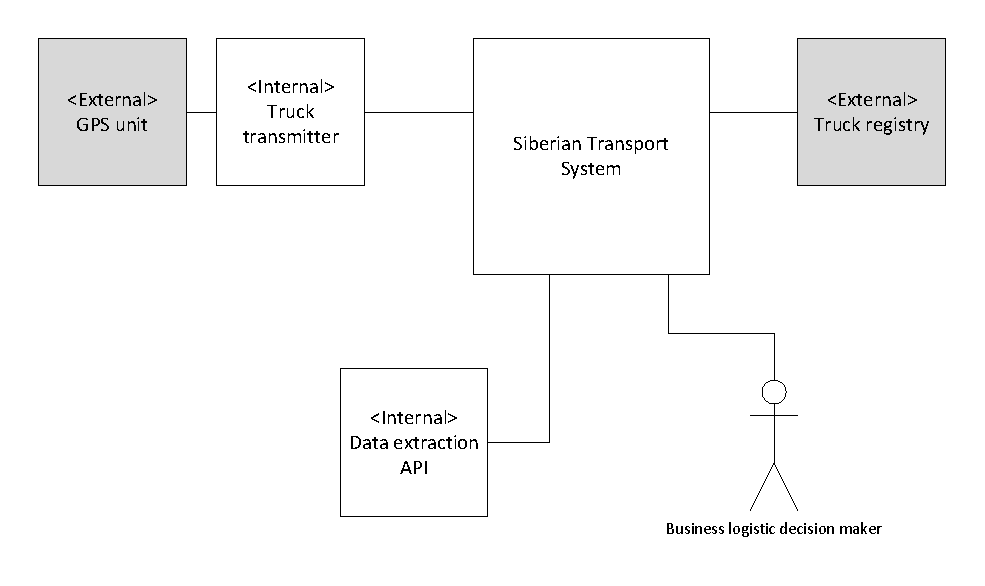
\includegraphics[width=\textwidth]{figures/sts_formal_context_diagram}\\
\end{center}
  \mycaption{Context diagram with information of externat and internal parts }

\begin{itemize}
\item The truck transmitters consist of a GPS unit, that gathers the trucks coordinates, and a sender unit, which will send the coordinates to our servers through a mesh-network. The hardware is a commodity-bought external system, but the software on the sender unit is internal.
\item The truck register is a system in which the Siberian trucking company's trucks are registered.  All the trucks will already be registered in this system, so data is imported from here to STS.  In the scope of our project, the truck register is an external system.  The trucks register sends a message to STS whenever a truck is added to the fleet, removed from the fleet, or reaches one of STC's central depots.
\end{itemize}


\subsection{Interaction scenarios}
\label{sec:inter-scen}

\begin{center}
  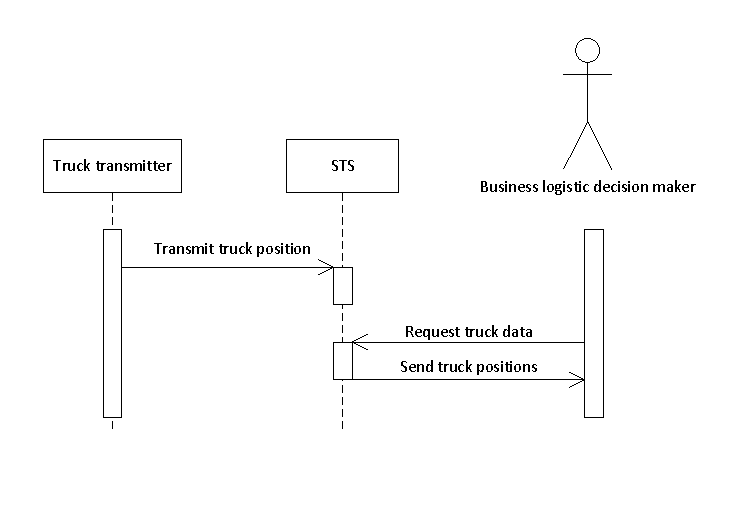
\includegraphics[width=\textwidth]{figures/interaction_scenario_1}\\
  \mycaption{Truck transmitters send positions to the server.  Later on, a user can make a query to see specific trucks or to see all trucks that fall behind schedule}
\end{center}



\section{Functional view}
\label{sec:functional-view}

\begin{center}
  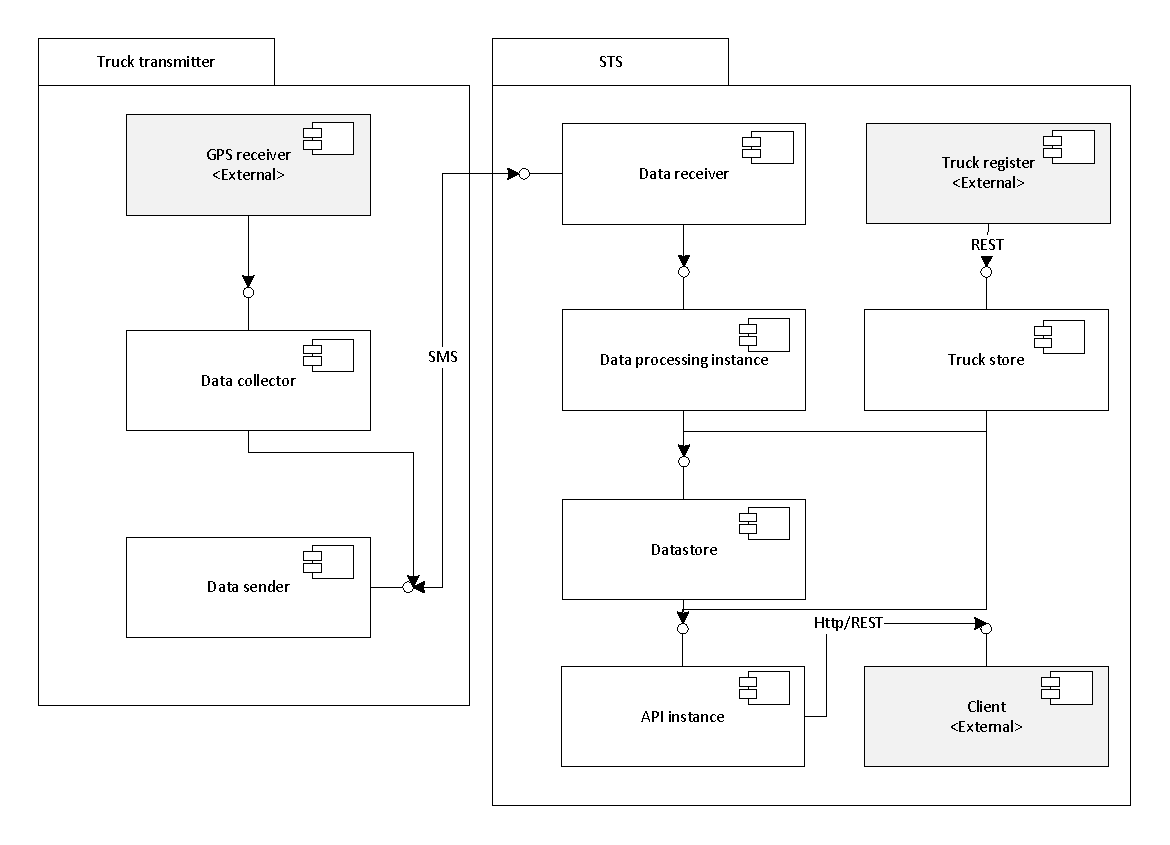
\includegraphics[width=\textwidth]{figures/functional_view}\\
  \mycaption{The figure shows the functional view for the truck transmitter and the Siberian Trucking System (STS) }
\end{center}


\subsection{Functional elements}
\label{sec:functional-elements}

\begin{center}
  \begin{tabular}[h!]{| >{\columncolor{gray}}p{0.28\textwidth} | p{0.65\textwidth} |}
    \hline
    Element name & GPS receiver\\
    \hline
    Responsibilities & acquire the current position of the truck \\
    \hline
    Interfaces -- inbound & none\\
    \hline
    Interfaces -- outbound & Data collector\\
   \hline
  \end{tabular}
\end{center}

\begin{center}
  \begin{tabular}[h!]{| >{\columncolor{gray}}p{0.28\textwidth} | p{0.65\textwidth} |}
    \hline
    Element name & Data collector\\
    \hline
    Responsibilities & Gather those positions that should be sent to the server\\
    \hline
    Interfaces -- inbound & GPS receiver\\
    \hline
    Interfaces -- outbound & Data sender\\
   \hline
  \end{tabular}
\end{center}

\begin{center}
  \begin{tabular}[h!]{| >{\columncolor{gray}}p{0.28\textwidth} | p{0.65\textwidth} |}
    \hline
    Element name & Data sender\\
    \hline
    Responsibilities & send truck positions encrypted via SMS to the server and get confirmation from the data receiver\\
    \hline
    Interfaces -- inbound & Data collector, Data receiver\\
    \hline
    Interfaces -- outbound & Data receiver\\
   \hline
  \end{tabular}
\end{center}

\begin{center}
  \begin{tabular}[h!]{| >{\columncolor{gray}}p{0.28\textwidth} | p{0.65\textwidth} |}
    \hline
    Element name & Data receiver\\
    \hline
    Responsibilities & Gather the positions from all the trucks, decrypt the messages and send confirmations to the trucks, when the data is received\\
    \hline
    Interfaces -- inbound & Data sender\\
    \hline
    Interfaces -- outbound & Data sender and Data processing instance\\
   \hline
  \end{tabular}
\end{center}

\begin{center}
  \begin{tabular}[h!]{| >{\columncolor{gray}}p{0.28\textwidth} | p{0.65\textwidth} |}
    \hline
    Element name & Data processing instance\\
    \hline
    Responsibilities & Send data to the datastore\\
    \hline
    Interfaces -- inbound & Data receiver\\
    \hline
    Interfaces -- outbound & Datastore and Truck store\\
   \hline
  \end{tabular}
\end{center}

\begin{center}
  \begin{tabular}[h!]{| >{\columncolor{gray}}p{0.28\textwidth} | p{0.65\textwidth} |}
    \hline
    Element name & Datastore\\
    \hline
    Responsibilities & Store all relevant data from the trucks\\
    \hline
    Interfaces -- inbound & Data processing interface, Truck register\\
    \hline
    Interfaces -- outbound & API instance\\
   \hline
  \end{tabular}
\end{center}

\begin{center}
  \begin{tabular}[h!]{| >{\columncolor{gray}}p{0.28\textwidth} | p{0.65\textwidth} |}
    \hline
    Element name & API instance\\
    \hline
    Responsibilities & Make data accessible for other external applications\\
    \hline
    Interfaces -- inbound & Datastore\\
    \hline
    Interfaces -- outbound & External client\\
   \hline
  \end{tabular}
\end{center}


\subsection{Functional scenarios}
\label{sec:functional-scenarios-1}

\begin{center}
  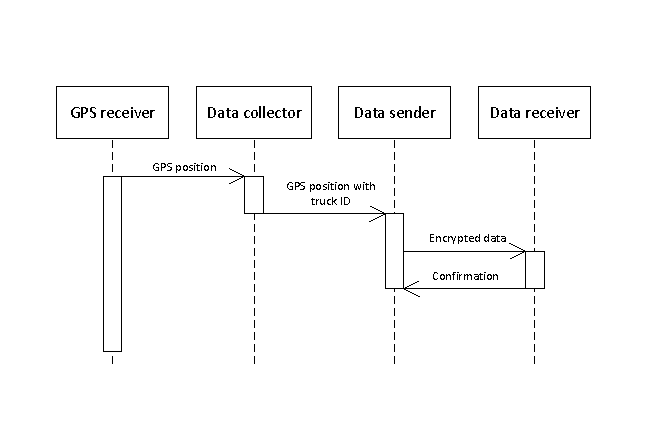
\includegraphics[width=\textwidth]{figures/functional_scenario}\\
  \mycaption{Truck transmitters send positions to the server end gets a confirmation when the data is received}
\end{center}

\subsection{System-wide processing}
\label{sec:syst-wide-proc}

The transmitters will often be out of reach for some network, therefore it is essential to be able to store and send the gathered data at a later point, when the truck again is within range of a network. When the transmitter sends data, it awaits a confirmation from the server before the data is registered as sent in the truck transmitter. If a transmitter hasn't sent a position in a considerable amount of time, when the truck is expected to be at a depot within transmission range, then a notification is raised in the system, to make a technician aware of a possible problem with the trucks transmitter. 


\section{Information view}
\label{cha:information-view}


The GPS receiver transmits GPS coordinates along with a timestamp.
This information is transmitted to the data collector, which filters
and aggregates the information, as well as tagging it with a truck ID.
These aggregations are sent to other truck transmitters in range, or
to the STS via the data sender if possible.  When the data has been
successfully transmitted to the STS, it is deleted from the truck
transmitter.

When truck position data is received by the STS, it becomes the
property of the system.  If it is to be saved (that is, if
cryptographic checks affirm its validity and the truck ID is of a
known truck), it will be stored in the data store component.  Data is
never deleted once stored.

When a truck is added or removed via the truck register, the truck ID
is stored or deleted from the truck store.  This data is always
accessible to the data processor and must be up to date.  Data never
flows from the data processor to the truck store.

The user-facing API uses data from the data store and provides an
aggregated view to its callers.  That is, data flows from the data
store to the API, never the other way.  Hence, the API does not allow
modification of data, it is read-only.

The data store is an unstructured NoSQL database (SimpleDB) provided
by the Amazon S3 platform.  The truck store is a relational database
using Amazon RDS.

Every HTTP request to the API is logged by the API provider.  Every
component failure is logged by the redundancy infrastructure
mechanism.

\subsection{Data structure}
\label{sec:data-structure}

\begin{center}
  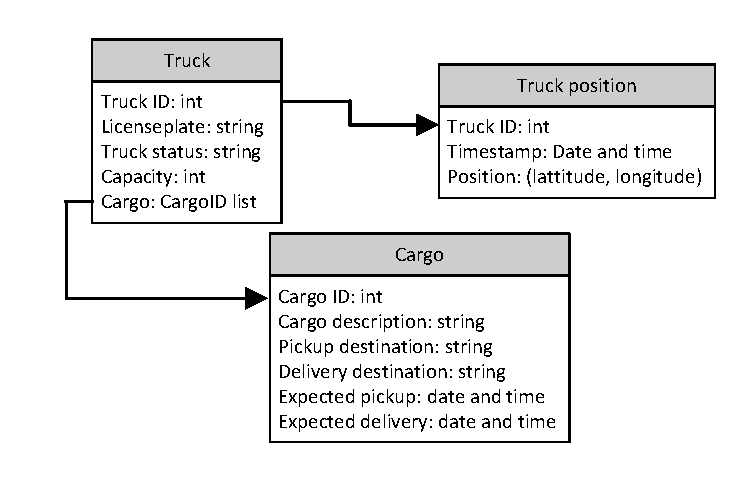
\includegraphics[width=\textwidth]{figures/Data_structure}\\
  \mycaption{System data structure}
\end{center}


The data store contains an unorganised set of tuples.  Each tuple
consists of a truck ID along with a timestamp and the trucks location
at that time. The truck store contains the truck data the system uses, which is gathered from the truck registry

\subsection{Data flow}
\label{sec:data-flow}

\begin{center}
  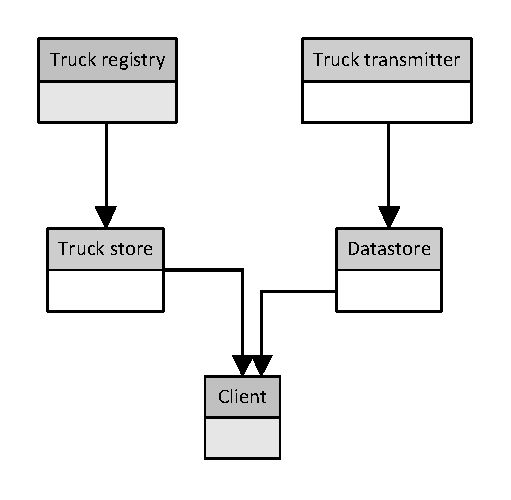
\includegraphics[width=0.5\textwidth]{figures/Data_flow}\\
  \mycaption{System data flow}
\end{center}
Whenever a truck notification event is received from the truck
register (for example, that a truck ID is added or removed), the truck
store is updated accordingly.  Transmitted positions are kept in the
datastore, and a client can access both via the API.

\subsection{Data ownership}
\label{sec:data-ownership}

\begin{tabular}{|c|c|c|c|c|c|c|}
\begin{sideways}\textbf{System}\end{sideways} & \begin{sideways}\textbf{Truck transmitter}\end{sideways} & \begin{sideways}\textbf{Data processor}\end{sideways} & \begin{sideways}\textbf{API}\end{sideways} & \begin{sideways}\textbf{Truck register}\end{sideways} & \begin{sideways}\textbf{Data store}\end{sideways} & \begin{sideways}\textbf{Truck store}\end{sideways} \\\hline
Raw truck data & writer & updater & reader & none & master & none \\\hline
Truck location & none & creator & reader & none & master & none \\\hline
Currently known trucks & none & reader & none & writer & none & master \\\hline
\end{tabular}

\subsection{Information lifecycles}
\label{sec:inform-lifecycl}

\begin{center}
  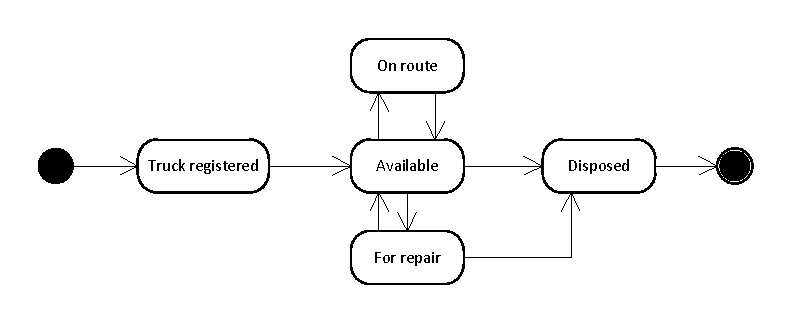
\includegraphics[width=\textwidth]{figures/Information_lifecycle}\\
  \mycaption{State diagram for a truck in the system}
\end{center}

Truck information is gathered from the truck registry, which means that this diagram isn't directly a part of our system, but a part of the external "truck registry". These state transitions will however impact on our system too, as changes to the truck in the truck registry will propagate to the "truck store" 

\subsection{Timeliness and latency}
\label{sec:timeliness-latency}


There are few explicit timeliness or latency requirements.  The
unavoidable latency involved in communicating from trucks to the STS
will dominate any other delays.

The only exception is the case where a new truck is added to the truck
register.  In that case, the knowledge that a truck has been added
must be propagated before that truck starts sending location
information, or it will be discarded.  This should not require any
particular engineering effort in the system: the users can add the
truck ID via the truck register several days before the truck is
actually put into service.

\subsection{Archive and retention}
\label{sec:archive-retention}

Records are never removed from the data store.  No explicit archiving
is necessary or performed, beyond that which is done automatically by
the database provider (Amazon SimpleDB).

\section{Concurrency view}
\label{sec:concurrency-view}


Each physical truck runs a single truck transmitter instance, which
contains three tasks: GPS reader, data collector and data sender.

The data and truck stores is distributed across several different
processes in order to provide redundancy and scability.

There is a 1:1 relationship between trucks and data processor tasks.
Each data processor is responsible for processing data from a single
truck.

The data receiver consists of a small (fixed) number of processes that
merely route truck data to the proper data processors.  If no task
processor is running for the given truck, it must be started.  If it
fails, it must be restarted.  See section \ref{sec:avail-resil} for
more on availability.

Each API request results in a logical task responsible for carrying
out the request.

\subsection{Concurrency model}
\label{sec:concurrency-model}

\begin{center}
  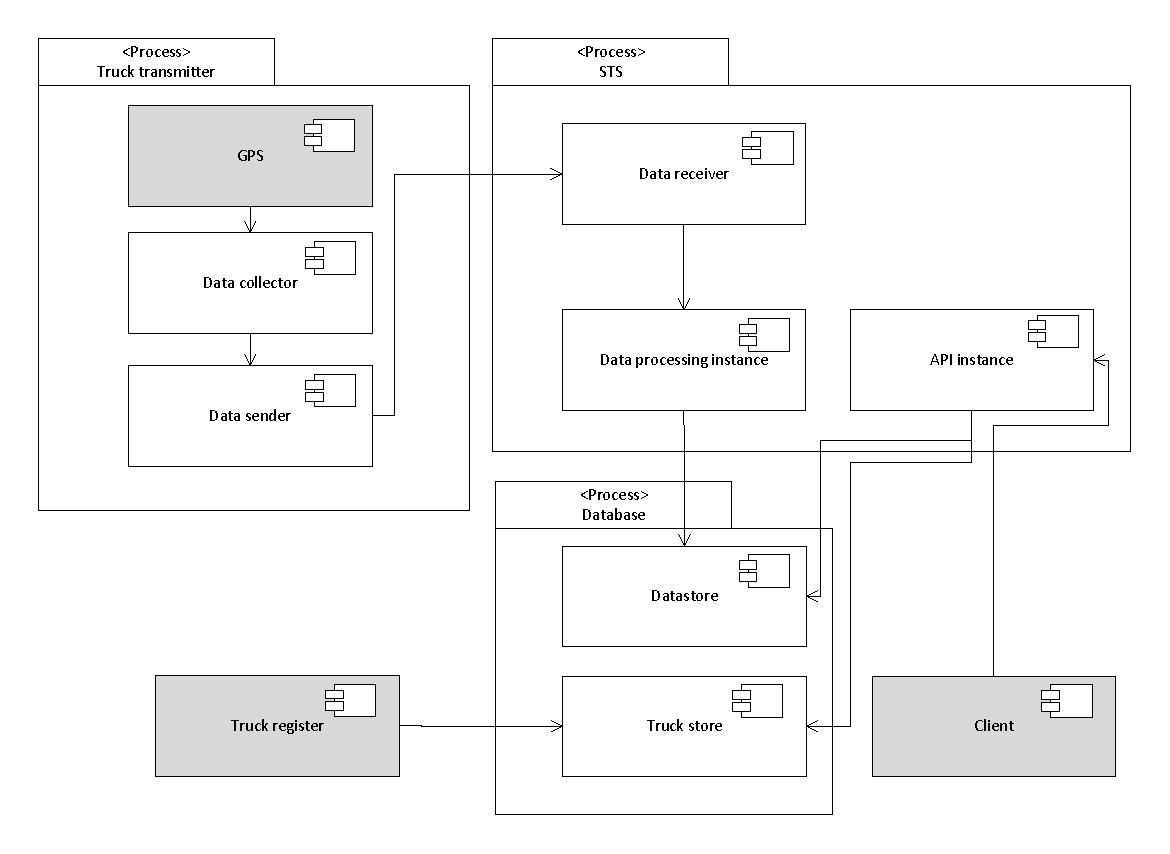
\includegraphics[width=\textwidth]{figures/concurrency_model}\\
  \mycaption{Concurrency model}
\end{center}

The truck transmitter is one process, that consists of the Data collectore and Data sender, which is placed on a physical device in the truck. Data is sent from the Data sender to the Data receiver. The Data receiver, Data processing instance and API instance all run on the server as individual processes. The Datastore and Truck store exists in a database process.

\subsection{State model}
\label{sec:state-model}


\begin{center}
  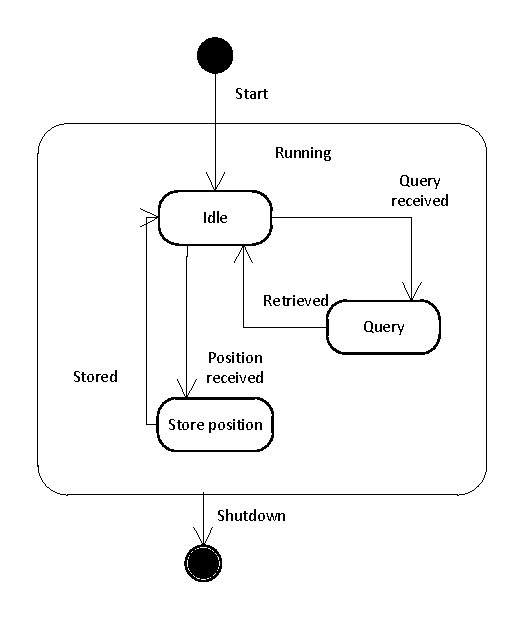
\includegraphics[width=0.7\textwidth]{figures/state_model}\\
  \mycaption{State model}
\end{center}

When the system is running, positions can be written to the database and queries can be processed.

\section{Deployment view}
\label{sec:deployment-view}

The STS will utilize Amazon EC2 for its data aggregation and processing, and
the datastore will be implemented using Amazon's SimpleDB nonrelational
database technology. The truck register in the system will utilize the Amazon
RDS service to access its database. To simplify deployment, the STS will
leverage the Amazon Elastic Beanstalk, an automated deployment utility that
leverages Amazon's AWS services to provide an automatically load-balanced and
scalable platform for development. The deployment will occur using a
centralized Git repository hosted by Amazon, and new versions of the software
will be automatically deployed when changes are pushed to this repository.
Amazon's software and hardware infrastructure will ensure the correct
deployment and scalability of the STS, as long as the code does not contain
critical errors or bugs.

The STS will use Ubuntu Server 12.04 images on Amazon EC2, and all server-side
code will be written in Python. The standard CPython Python interpreter will be
used to run the STS, and all HTTP-based communications will be handled using the
Apache webserver. Since the STS will leverage Amazon's SimpleDB and RDS database
platforms, no additional database software will be required on the EC2
instances.

\subsection{Runtime platform model}
\label{sec:runt-platf-model}


\begin{center}
  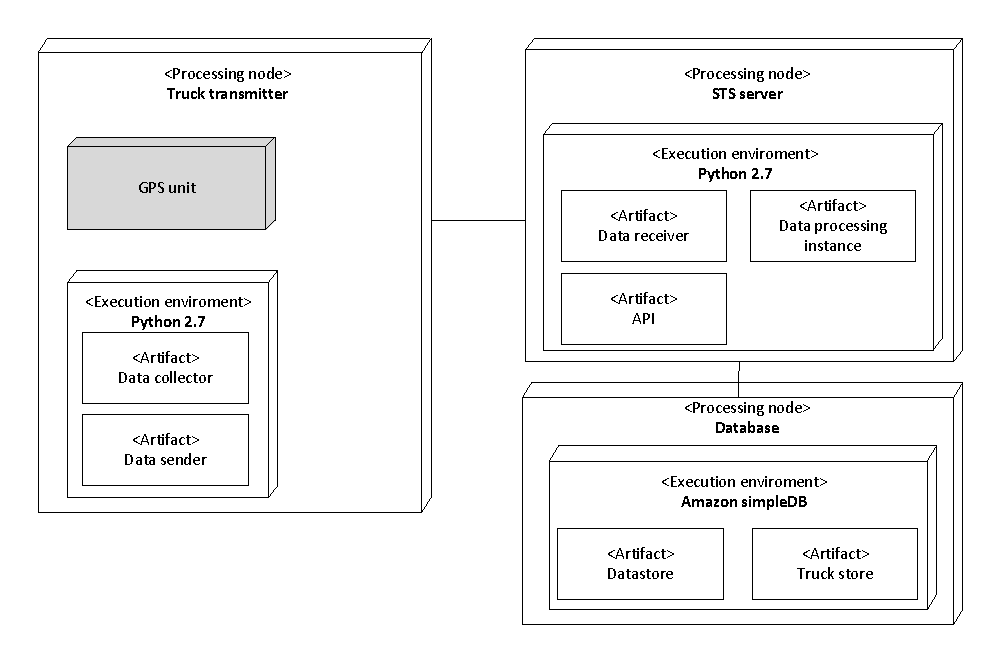
\includegraphics[width=\textwidth]{figures/Runtime_platform_model}\\
  \mycaption{Deployment model}
\end{center}
 The truck transmitter gets data from an external GPS unit, and sends data to the server via SMS or MESH network. The server consists of an Amazon EC2 server running Ubuntu 12.04 and a Amazon simpleDB for data storage.

\subsection{Software dependencies}
\label{sec:softw-depend}


\begin{center}
\begin{tabular}{c|c|c}
  \textbf{Dependency} & \textbf{Version} & \textbf{Depends on} \\\hline
  Ubuntu & 12.04 & \\
  Python & 2.7 & \\
  Boto (interface to AWS) & 2.6.0 & Python 2.6 or 2.7 \\
  PyCrypto & 2.6 & Python 2.x or 3.x
\end{tabular}
\end{center}

Additionally, various non-runtime systems will be needed for
deployment and development, such as Git and Pip.  The specifics of
these are left at the discretion of the developers.

\subsection{Network model}
\label{sec:network-model}


The physical network model is automatically managed by the Amazon WS
platform.  This implies that we cannot provide any guarantees beyond
the service level agreement, and further robustness must be
implemented at the software level.

Communication between trucks and the STS server is done through the
mobile telephone network by sending SMS messages.

Communication between trucks is done through a short-range radio
transmitter, forming a mesh network.

\section{Development view}
\label{sec:development-view}


\subsection{Module structure}
\label{sec:module-structure}


\begin{center}
  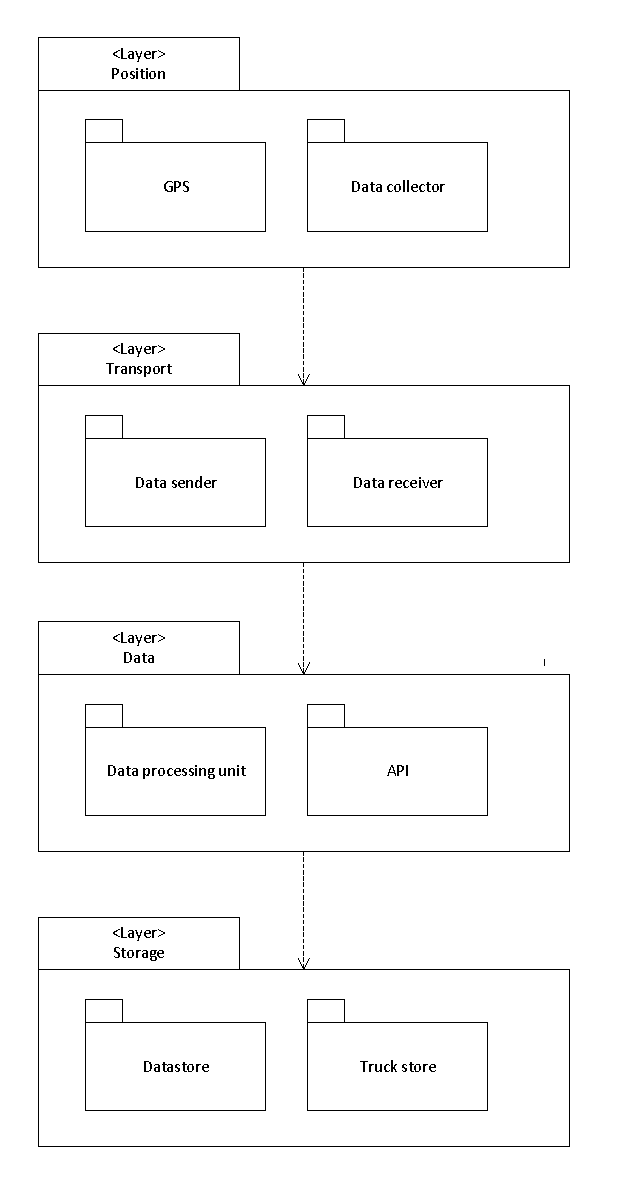
\includegraphics[width=0.7\textwidth]{figures/module_structure}\\
  \mycaption{Module structure diagram}
\end{center}

\subsection{Common design}
\label{sec:common-design}

Logging and error-handling will be tracked using the standard Python logging 
module. The logging module on EC2 will be configured such that error logs from
the STS will be saved to the Amazon SimpleDB service for review. Similarly,
traces in the event of an exception will also be logged to SimpleDB. All 
data encryption within the STS will be handled through the PyCrypto library.

\subsection{Standards for design, code, and test}
\label{sec:stand-design-code}

The STS will be developed using the Python programming language, and each of
the functionalities contained within the system will be separated into separate
Python modules. The code will follow the guidelines set in PEP-8, the coding
style recommended by the Python developer community. Every public API contained
within a module of the STS must contained an appropriate unit test either
embedded within its documentation using the doctest framework, or in a separate
Python file using the unittest module provided with the Python programming
language.

\subsection{Codeline organization}
\label{sec:codel-organ}

Dependencies on third-party modules and libraries will be monitored using PIP,
the Python package manager, and each discrete module in the STS must have a
file named "requirements.txt" with an appropriately formatted list of modules
and the minimum version number required for the proper functioning of the STS
software. Deployment and version control will be managed through Git, and the
deployment to Amazon EC2 will be handled through a centralized Git repository
managed using Amazon Elastic Beanstalk. The STS modules will be separated into
three directories: "static," "src," "docs," and "libs." The "static" directory
will contain any static files related to the STS system, the "src" directory
will hold the Python modules of the STS (each module will be contained within
its own subdirectory with an initialization file), the "docs" directory will
contain all documentation associated with the STS, and the "libs" directory
will contain all of the third-party Python modules necessary to run the STS.

\section{Operational view}
\label{sec:operational-view}


\subsection{Installation and migration}
\label{sec:inst-migr}


The installation of the STS will be handled through the Amazon Elastic Beanstalk
platform. To install the STS, a new project must be created using the AWS
control panel. Once Amazon creates a central Git repository for the project, the
STS code will need to be configured with the appropriate authentication details
for the AWS account being used, including the SimpleDB and RDS databases being
used. After the STS code is configured, it can be installed by pushing to the
master branch of the Elastic Beanstalk Git repository. All further deployments
of the STS may be handled through Git.

To separate the ongoing version control of the STS with its deployment, the STS
development team will be required to push changes to two separate Git
repositories. The first repository, hosted externally on Github will contain
potentially-unstable development code. Once the code in this repository matures
and is thoroughly tested, the changes can be easily pushed to the second
repository hosted by Amazon. Due to the simplified branching and merging
available within Git, bug fixes can be quickly and efficiently deployed to EC2,
while larger changes that require more testing can be re-integrated later.

\subsection{Operational configuration management}
\label{sec:oper-conf-manag}


The configuration for the STS will be related to the implementation of AWS API's
used by the system, including RDS, SimpleDB, EC2, and Elastic Beanstalk. The
Python library Boto provides a simple interface for interacting with and
configuring the AWS API's, so the configuration for the STS will be housed in a
Python module named "configuration." This module should contain the relevant
AWS API access keys and connection details for the SimpleDB and RDS database
systems.

\subsection{System administration}
\label{sec:syst-admin}


Amazon will provide all hardware-related systems administration, and EC2 
provides a 99.95 percent uptime guarantee. Although hardware failure alone is
unlikely, programmatic errors are possible, so systems administrators must
maintain at minimum a daily backup of the STS data in the event of accidental
data deletion or corruption. To ensure the optimal functioning of the STS,
systems administrators must also regularly monitor the health of the system by
using automated monitoring tools, such as New Relic.

\subsection{Provision of support}
\label{sec:provision-support}


The STC will have a team of IT professionals responsible for providing basic
support for the STS. Any problems related to the general use of the system will
be handled by this IT department. If the problem is found to be an issue with 
the STS itself, the issue will be escalated to the in-house development team of
the STC, which is in charge of maintaining and administering the STS system. If
the problem is then found to be related to the infrastructure of the system, 
the development team will contact Amazon AWS support staff.

\chapter{System qualities}
\label{cha:system-qualities}
\thispagestyle{fancy}

\section{Performance and scalability}
\label{sec:perf-scal}
In this section we present a table of the performance requirements for the expected scale of the system and reason by what means the requirements can be met and why these requirements are possible to uphold.

\begin{center}
  \begin{longtable}[h!]{| p{0.4\textwidth} | p{0.5\textwidth} |}
    \hline
    \rowcolor{gray}
    Requirement & How met \\
    \hline
    \hline
    Average response time for the STS API should be less than 100ms under a
    load of up to 20 requests per second & Amazon Elastic Beanstalk will
    automatically start and stop additional EC2 instances according to the
    level of load experienced by the STS. The configuration of Elastic
    Beanstalk will ensure that the response time remains low. \\
    \hline
    Average response time for the data aggregator should be less than 50ms
    under a load of up to 200 requests per second & the implementation of
    Amazon Elastic Beanstalk will mimic the implementation of the API, but
    Elastic Beanstalk will be configured to suit the data aggregator and
    produce a sub-50ms response time. \\
    \hline
    The datastore should respond to queries for up to 10,000 separate data
    points in under 1,000ms, regardless of the total size of the database & the
    datstore will be implemented on top of SimpleDB, which has predictable
    performance characteristics that do not change based on the total amount of
    data in the database. \\
    \hline
    Verifying the existence of a truck in the truck store should require
    less than 15ms of time & the truck register will act as a cache for the
    truck store, and the truck register will be implemented on top of the
    Amazon RDS platform with aggressive and distributed in-memory caching. \\
    \hline
    Network latency between the datastore, truck register, data aggregator,
    and API endpoints must be less than 5ms & AWS has latencies of
    approximately 1ms between different availability zones and less than 1ms
    when communicating within an individual availability zone. \\
    \hline
    Although the STS will be ready occasionally delayed SMS delivery, SMS
    messages from the trucks should ideally arrive within 5 seconds of being
    sent & the mobile operator or virtual network provider must guarantee a low
    latency for SMS messages. It is assumed that the STC can negotiate an
    appropriate contract. \\
    \hline
    Although the STS can appropriately handle the event in which an SMS is
    not delivered from a truck (no data will be recorded), SMS messages should
    ideally have a minimum of a 99 percent delivery rate & it is assumed that 
    the STC can negotiate an appropriate contract with a network provider. \\
    \hline
    The server infrastructure of the STS must have at least 99.9
    percent uptime & Amazon's AWS infrastructure guarantees 99.95 percent
    uptime. \\
    \hline
 \end{longtable}
\end{center}


\section{Security}
\label{sec:security}

\instructions{
For each of the main, security requirements, explain how the system
will meet the requirement. Define (or reference) the threat model,
security policy and security design that have been used as part of
applying this perspective.
}

Much of the internal security of the STS server is delegated to our
deployment infrastructure (Amazon WS).  This section is mostly
concerned with issues arising from the parts of STS using unsecured
networks or interacing with the external world.  The following table
summarises our security requirements, we provide motivation for our
requirements in subsections \ref{sec:acp} and \ref{sec:threats}.

\begin{center}
  \begin{tabular}[h!]{| p{0.4\textwidth} | p{0.5\textwidth} |}
    \hline
    \rowcolor{gray}
    Requirement & How met \\
    \hline
    \hline
    Truck position information must be kept confidential. &
    Position information must be encrypted whenever transmitted across unsafe networks (wireless meshes or the SMS network).
    \\
    \hline
    Truck communication must not be forgeable. &
    Every truck possesses its own unique private key.  All positions generated by the truck will be encrypted with that key.  The STS server will reject any truck position not encrypted with a known key. \\
    \hline
    Only authorised users may obtain truck information via the API. &
    An API key must be used to authenticate any requests.
    \\
    \hline
    Canonical truck position information must not be forgeable. &
    The truck register must prove its validity with a cryptographic signature.
    \\
    \hline
 \end{tabular}
\end{center}

\subsection{Access control policy}
\label{sec:acp}

Much of the system is automated, or only accessed by other systems, so
the principals are generally not persons.  Since we store very few
kinds of data, and have only one user class, our access control policy
is particularly simple.

\begin{center}
  \begin{tabular}[h!]{|p{0.2\textwidth}|p{0.2\textwidth}|p{0.2\textwidth}|p{0.2\textwidth}|}
    \hline
    \rowcolor{gray}
    Principal & Truck positions & Truck existence & Canonical truck location \\
    \hline
    \hline
    API user & Read-only operations & None & None \\
    \hline
    Truck register & None & Write-only operations & Write-only operations \\
    \hline
    Truck & Write-only operations & None & None \\
    \hline
  \end{tabular}
\end{center}

\subsection{Threat identification}
\label{sec:threats}

\renewcommand{\labelenumi}{\textbf{\arabic{enumi}.}}
\renewcommand{\labelenumii}{\textbf{\labelenumi\arabic{enumii}.}}
\renewcommand{\labelenumiii}{\textbf{\labelenumii\arabic{enumiii}.}}

\begin{description}
\item[Goal: ] Determine the location of a truck.
  \begin{enumerate}
    \item Extract information from the STS server itself.
      \begin{enumerate}
        \item Access the data store directly.
          \begin{enumerate}
          \item Guess database password.
          \item Exploit software vulnerability.
          \end{enumerate}
        \item Access data through API via obtained API key.
          \begin{enumerate}
            \item Crack API key.
            \item Obtain API key from valid user.
          \end{enumerate}
        \item Use social engineering to coerce a valid user to provide
          the information.
      \end{enumerate}
    \item Intercept truck communication containing the position of
      another truck.
    \item If you know the position history truck $T_{1}$, and
      communications from truck $T_{1}$ contains truck positions from
      truck $T_{2}$, the attacker can deduce that they must have met
      recently.
  \end{enumerate}
\item[Handling: ] The truck IDs in truck positions are encrypted using
  assymetric key cryptography.  Each truck has a unique keypair, the
  transmitter containing only the public key.  Every truck position is
  encrypted with this key, and decrypted with the private key by the
  STS.  Without the private key, you can tell neither which truck it
  is, nor where it has been.

  We assume that the standard cryptographic algorithms will not be broken.
\item[Goal: ] Forge location of a truck.
  \begin{enumerate}
  \item Obtain the private key of the truck and use it to send
    properly signed truck positions.
    \begin{enumerate}
      \item Gain physical access to the truck transmitter itself.
    \end{enumerate}
  \item Access the data store directly.
  \end{enumerate}
\item[Handling: ] Obtaining physical access to a hardware device is
  not easy.  The data store uses a secure (standard) authentication
  mechanism.
\item[Goal: ] Overload the mesh network.
  \begin{enumerate}
  \item Flood trucks with forged positions from other, fictitious
    trucks.
  \end{enumerate}
\item[Handling: ] A truck transmitter must only store truck positions
  signed by a central key known to all trucks.  This key is relatively
  easily obtained, by hijacking any truck in the fleet, and takes a
  long time to replace, since every truck transmitter must be
  modified.  This is still acceptable, as this is only a mild
  denial-of-service attack.
\end{description}

\section{Availability and resilience}
\label{sec:avail-resil}

There are three types of service, with associated service levels.

\begin{description}
\item[API requests: ] normal, no service.
\item[Truck store: ] normal, read-only, no service.
\item[Transmitting data from trucks: ] normal, STS down (trucks can
  still send to each other).
\end{description}

The services do not always function independently of each other.  If
the truck store is down, data cannot be received from trucks to the
STS, as the validity of truck positions cannot be verified.  On the
other hand, if we take care that data, once stored, cannot be lost,
and let truck transmitters retain data until the STS is able to store
it, we will not suffer information loss.

The API requests only need to be under normal operation during 
business hours of the STC (8am - 4pm on business days) with an
availability of 99.9 percent. The truck store must maintain normal
operation at least 95 percent of the time during business hours
of the STC, and must maintain at least read-only access 99.9 percent
of the time during business hours. The STS server must be able to receive data
from any active STC trucks with a 99.9 percent availability between 5am and 8pm, as it is expected, that most trucks will be operational in this period of time. 

\begin{center}
  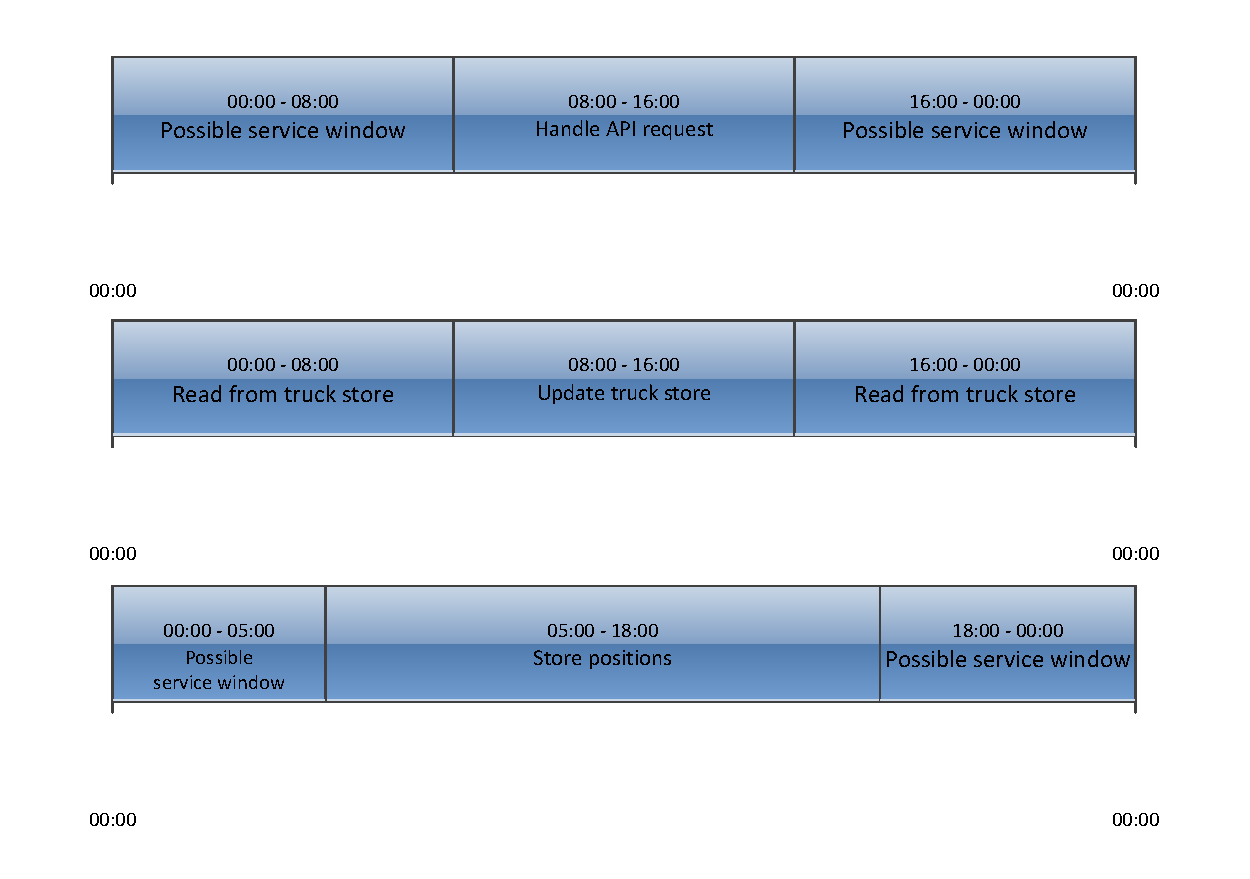
\includegraphics[width=1\textwidth]{figures/functional_availability}\\
  \mycaption{Availability of STS}
\end{center}

The overall system defines the following service levels.

\begin{description}
\item[Normal operation: ] Data can be received from the trucks, new
  trucks can be added.
\item[Autonomic operation: ] As in normal operation, but the API is
  not accessible and the truck store is read-only.
\item[Read-only operation: ] Only the API is available.  No new data
  is stored, but old data can still be queried.
\item[No service: ] No part of the system is reachable or functional.
\end{description}

\subsection{Platform availability}

The STS is deployed on Amazon WS, using Amazon S3 for virtual machine
instancs and Amazon EasyDB for data storage.  According to the Service
Level Agreement\footnote{\url{http://aws.amazon.com/ec2-sla/}}, we can
expect 99.95\% uptime per availability zone.  This does not cover
the reliability of an individual instance, but only our ability to
start new ones in case an existing instance crashes.  As a
consequence, the STS must be able to automatically restart components
running on virtual machine instances that become unreachable.

\subsection{Availability scenarios}

\begin{center}
  \begin{tabular}[h!]{| >{\columncolor{gray}}p{0.28\textwidth} | p{0.65\textwidth} |}
    \hline
    Scenario reference & AS1 \\
    \hline
    Overview & Availability of truck position processing. \\
    \hline
    System environment & The system is operating normally. \\
    \hline
    Environment change & A data processor task fails. \\
    \hline
    Required system response & A new data processor task must be started. \\
    \hline
  \end{tabular}
\end{center}
\begin{center}
  \begin{tabular}[h!]{| >{\columncolor{gray}}p{0.28\textwidth} | p{0.65\textwidth} |}
    \hline
    Scenario reference & AS2 \\
    \hline
    Overview & Resilience in the face of truck store failure \\
    \hline
    System environment & The truck store is operating normally \\
    \hline
    Environment change & The truck store becomes unreachable \\
    \hline
    Required system response & Data processors for already known trucks must keep processing data received from truck transmitters. \\
    \hline
  \end{tabular}
\end{center}

\begin{center}
  \begin{tabular}[h!]{| >{\columncolor{gray}}p{0.28\textwidth} | p{0.65\textwidth} |}
    \hline
    Scenario reference & AS3 \\
    \hline
    Overview & Resilience in the face of STS failure. \\
    \hline
    System environment & The STS is operating normally. \\
    \hline
    Environment change & The STS becomes inaccessible to the truck transmitters. \\
    \hline
    Required system response & Truck transmitters must store data points locally, intelligently remove data points close in time, to conserve limited space.  As soon as the STS is once again accessible, the data must be transmitted.  \\
    \hline
  \end{tabular}
\end{center}

\begin{center}
  \begin{tabular}[h!]{| >{\columncolor{gray}}p{0.28\textwidth} | p{0.65\textwidth} |}
    \hline
    Scenario reference & AS4 \\
    \hline
    Overview & Able to restore data store from backup. \\
    \hline
    System environment & The data store is operating normally. \\
    \hline
    Environment change & The contents of the data store are lost due to a technical fault at Amazon. \\
    \hline
    Required system response & The data store must be manually recreated using an externally stored (and recent) backup.  Such a backup must hence exist. \\
    \hline
  \end{tabular}
\end{center}

\begin{center}
  \begin{tabular}[h!]{| >{\columncolor{gray}}p{0.28\textwidth} | p{0.65\textwidth} |}
    \hline
    Scenario reference & AS5 \\
    \hline
    Overview & Able to recreate truck store from truck register. \\
    \hline
    System environment & The truck store is operating normally. \\
    \hline
    Environment change & The contents of the truck store are lost due to a technical fault at Amazon. \\
    \hline
    Required system response & The truck store is manually repopulated from the truck register. \\
    \hline
  \end{tabular}
\end{center}

\section{Evolution}
\label{sec:evolution}

The STS is designed to meet an immediate, static business need of the
company.  As the STS is mostly a data aggregator, most new features
will be implemented as new systems that consume data generated by the
STS.  Hence, we present few evolutionary perspectives.

\begin{center}
  \begin{tabular}[h!]{| p{0.4\textwidth} | p{0.5\textwidth} |}
    \hline
    \rowcolor{gray}
    Requirement & How met \\
    \hline
    \hline
    1. It must be possible to add extra data processing and aggregation
    algorithms to the system based on the needs of the STC in the future &
    Data processing functionality will be separated into loosely coupled Python
    modules such that additional modules may be easily integrated. \\
    \hline
    2. It must be possible to add new ways of querying the data should the need
    arise & The datastore will have an index that can be updated to support more
    complex queries as necessary. Updating the index may take a substantial amount
    of time. \\
    \hline
 \end{tabular}
\end{center}


\instructions{
Explain the evolution requirements.

Define the evolutionary dimensions that are relevant to the system.

Explain  how the system will meet the requirements, taking into
account the likelihood of each type of evolution occurring (explaining
how the probabilities were arrived at) and referring to the design
work performed as part of applying his perspective.
}

\begin{center}
  \begin{tabular}[h!]{| p{0.45\textwidth} | c | c | c |}
    \hline
    \rowcolor{gray}
    Requirement & Magnitude & Likelihood & Timescale \\
    \hline
    \hline
    It must be possible to add other communication networks between trucks and server. & M & M & L\\
    \hline
    The system must be extended for marketing as a generic truck tracking system, usable by other trucking companies as well. & H & M & L\\
    \hline
    Support for non-Amazon deployment platforms must be added. & H & L & L\\
    \hline
 \end{tabular}
\end{center}

The STS has a very simple architecture, meaning that extending its
functionality is easy.  This was not an aim of the original design,
however, but a fortunate consequence of its simplicity.  On the other
hand, we explicitly decided to make heavy use of facilities provided
by Amazon's cloud platform, making future porting efforts very
difficult.

\section{Other qualities}
\label{sec:other-qualities}

\subsection{Accessibility}
\label{sec:accessibility}

\instructions{
Explain how the system meets any accessibility requirements (if any).
}

\subsection{Internationalisation}
\label{sec:internationalisation}

\instructions{
Explain how the system meets any internationalisation (or
localisation) requirements (if any).
}

\subsection{Location}
\label{sec:location}

\instructions{
Explain how the system meets any requirements for the geographical
location(s) it is to be installed in (if any).
}

\subsection{Regulation}
\label{sec:regulation}

\instructions{
Explain how the system meets any regulatory requirements (if any).
}

\subsection{Usability}
\label{sec:usability}

\instructions{
Explain how the system meets any usability requirements (if any).
}

\appendix

\chapter{Architecture backlog}
\label{cha:architecture-backlog}
\thispagestyle{fancy}

\instructions{ Maintain a \emph{backlog} listing needs you have,
  issues and problems you have to solve, ideas for future design
  decisions etc. Note actions that you need to take and update the
  backlog as actions are completed:

\bigskip
Actions

\begin{itemize}
\item Decide on which Android version to target
\item ...
\end{itemize}

Done

\begin{itemize}
\item Create an architectural prototype using java.nio for increased
  scalability

\end{itemize}


}

\chapter{Architecture evaluation}
\label{cha:arch-eval}
\thispagestyle{fancy}

\instructions{
Describe the architectural evaluation that you performed, cf. Chapter
14 of~\citet{rozanski2011software} including what you learned about
your architecture design.
}

\chapter{Architecture skeleton}
\label{cha:arch-prot}
\thispagestyle{fancy}
\instructions{ 
Describe the architecture skeleton that you developed
  including how to download and run it.
}





% 
% Bibliography
% 
\bibliography{architectural_design}
\bibliographystyle{apalike}

\end{document}
